\chapter{Covert Channel Attacks}

\section{Cache channels on GPGPU}

GPGPUs have a massively parallel architecture which allows for SIMT workloads
to efficiently run. Apart from graphics and display use-cases, GPGPUs are
being used for parallel computation using frameworks like CUDA and OpenCL.
GPGPUs in cloud services are specifically designed for such computational
use-cases. Nvidia GPGPUs have recently started to support concurrent kernel
execution at SM level, which allows multiple programs to simultaneously use
the GPGPU resource. In this shared context, one must look at side channels
which can be exploited.

\begin{figure}[h]
\centering
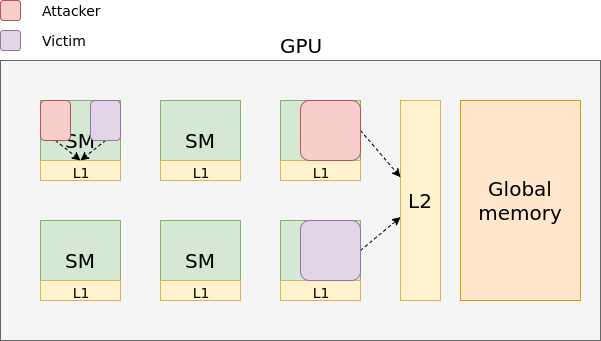
\includegraphics[width=0.7\textwidth]{gpgpu}
\caption[Memory layout of GPGPU]{GPGPU memory layout.
Attacker and Victim colocation allows using L1 and L2 caches as side channels.}
\label{fig:gpgpu}
\end{figure}

The structure of GPGPU memory layout is shown in \Figref{fig:gpgpu}. Every SM
contains a private L1 cache, and all SMs share an L2 cache. The Global memory
contains multiple types of memory division like Constant memory, Texture
memory etc. Concurrent kernel execution allows co-location of different
kernels on same SM. Due to resource constraints, kernels could also run on two
different SMs simultaneously. The first case allows attacker to use L1 cache
as side channel, and in the second case attacker has to use L2 cache.

Mounting a side channel attack on AES is possible on GPGPU because of existing
implementations of AES for GPGPU. However, there are not many cases where
encryption algorithms are run on GPGPUs. So these side channels are used as
covert channels instead. Covert channels use the same methods as side channel
but they are used to set up communication between two malicious programs. Such
covert channels can be useful to leak data to third parties without the OS or
hardware detecting malicious behaviour.

\begin{figure}[h]
\centering
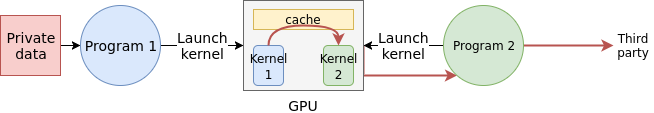
\includegraphics[width=\textwidth]{covert_channel}
\caption[Covert channel on GPGPU]{Structure of covert channel via GPGPU.}
\label{fig:gpgpu}
\end{figure}

Naghibijouybari et al in \Citeref{covert_gpgpu} achieve communication speed of
over 4Mbps using a combination of L1 cache contention and SFU contention as
covert channels on multiple Nvidia GPGPU architectures. They have used the
inherent parallelism in GPGPUs to multiply the speed of the created covert
channels by opening parallel communication channels on each SM.

A critical part of their attack is reverse engineering various parameters of
GPGPU architecture. To use caches as a side channel, we need to know all
parameters of the cache structure. We also need to know of the warp scheduling
policy to control colocation of two different kernels on same SM.

%\section{Reading kernel memory via cache covert channel on CPU}

% TODO Meltdown and Spectre
